\section{Desgin}

\subsection{Dataflow Shell Scripting}

\begin{figure}[htp]
\centering
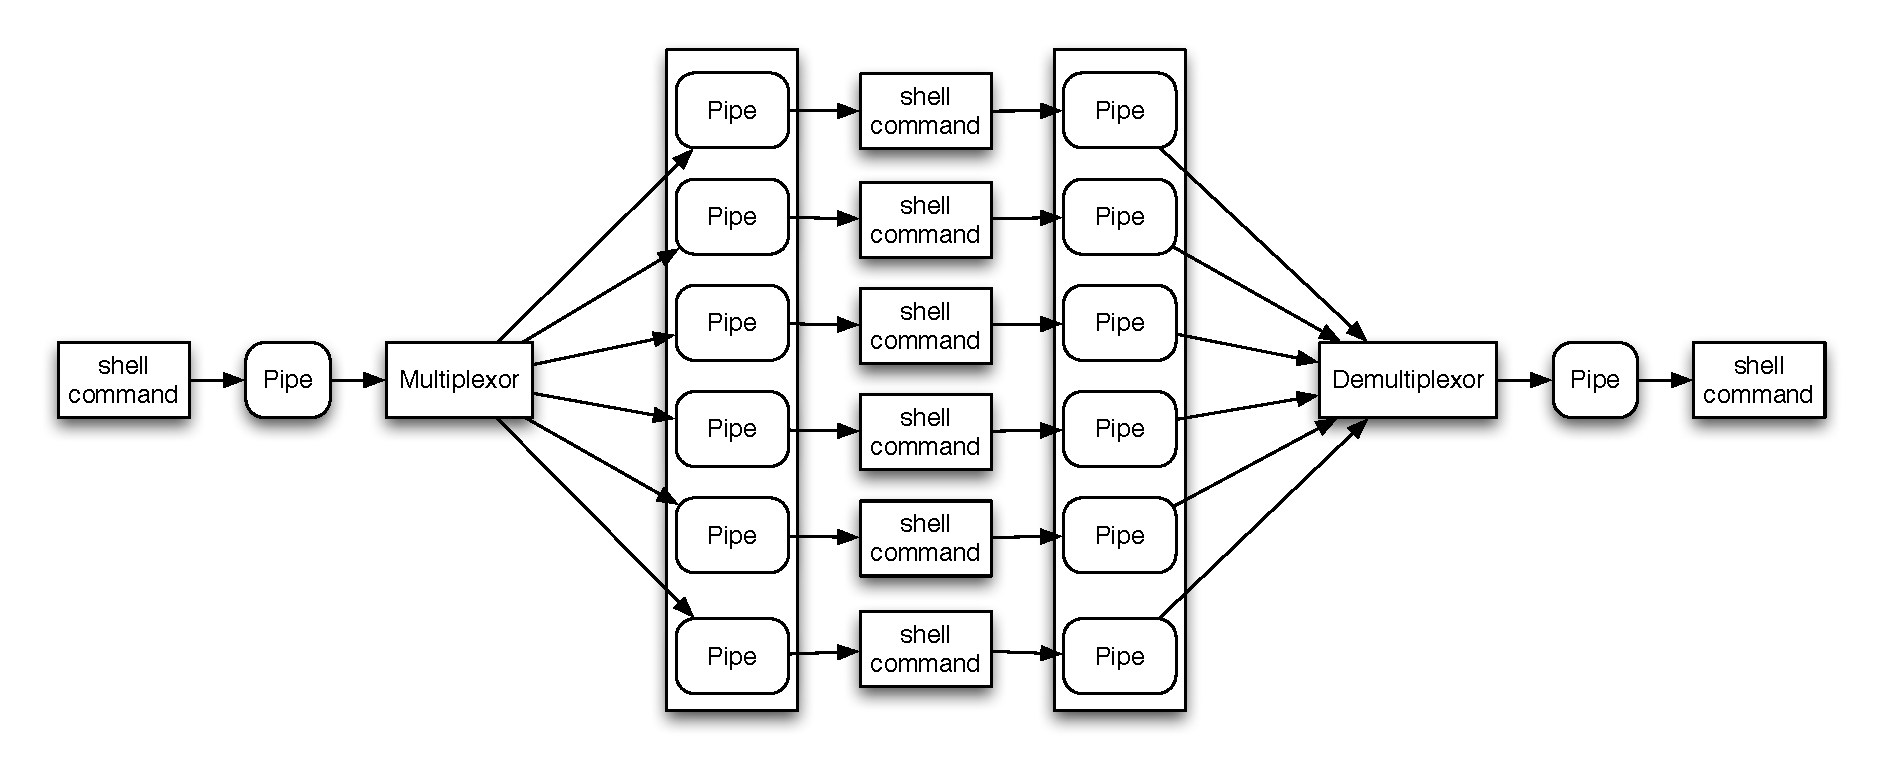
\includegraphics[width=3in]{pipestruct.eps}
\caption{The structure of the PUSH shell}
\label{fig:pipestruct}
\end{figure}

We have added two additional pipeline operators to a traditional UNIX shell,
a multiplexing fan-out(\verb!|<![\emph{n}]), and a coalescing fan-in(\verb!>|!).
 
This combination allows PUSH to distribute I/O to and from multiple
simultaneous threads of control.
The fan-out argument \emph{n} specifies the desired degree of parallel
threading.  If no argument is specified, the default of spawning a new
thread per record (up to the limit of available cores) is used.  This can
also be overriden by command line options or environment variables.
The pipeline operators provide implicit grouping semantics allowing natural
nesting and composibility.
While their complimentary nature usually lead to symmetric
mappings (where the number of fan-outs equal the number of fan-ins), there is
nothing within our implementation which enforces it.
Normal redirections as well as application specific sources and sinks
can provide alternate data paths.
Remote thread distribution and interconnect are composed and managed
using synthetic file systems in much the same manner as Xcpu,\cite{xcpu}
pushing the distributed complexity into the middleware in an language and
runtime neutral fashion.

PUSH also differs from traditional shells by implementing native support for
record based input handling over pipelines. This facility is similar to the
argument field separators, IFS and OFS, in traditional shells which use a
pattern to determine how to tokenize arguments. PUSH provides two variables,
ORS and IRS, which point to record separator modules. These modules
(called multiplexors in PUSH) split data on record boundaries, emitting
individual records that the system distributes and coalesces.

The choice of which \emph{multipipe}, an ordered set of pipes, to target is
left as a decision to the module.
Different data formats may have different output requirements.Demultiplexing from a multipipe is performed by creating a many to one
communications channel within the shell. The shell creates a reader processes
which connects to each pipe in the multipipe. When the data reaches an
appropriate record boundary a buffer is passed from the reader to the shell
which then writes each record buffer to the output pipeline.

An example from our particular experience, Natural Language Processing, is
to apply an analyzer to a large set of files, a "corpus". User programs go
through each file which contain a list of sentences, one sentence per line.
They then tokenize the sentence into words, finding the part of speech and
morphology of the words that make up the sentence.
This sort of task maps very well to the DISC model. There are a large number of
discrete sets of data whose order is not necessarily important. We need to
perform a computationally intensive task on each of the sentences, which are
small, discrete records and ideal target for parallelization.

PUSH was designed to exploit this mapping. For example, to get a histogram of
the distribution of Japanese words from a set of documents using chasen,
a Japanese morphological analyzer, we take a set of files containing sentences
and then distribute them to a cluster of machines on our network. The command
is as follows:
\begin{verbatim}
push -c '{
  ORS=./blm.dis  du -an files |< xargs os \\
   chasen | awk '{print \$1}' | sort | uniq -c \\
   >| sort -rn
}'
\end{verbatim}

The first variable, ORS, declares our record multiplexor module, the intermediar
y
used to ensure that the input and output to distributed pipes are correctly
aligned to record boundaries. du -n gives a list of the files (note that our
du is a bit different from the canonical UNIX du, it replaces much of find's
functionality) which are then "fanned out"(\verb!|<!) using a combination
of a multipipes, and a \emph{multiplexor}
which determines which pipes are the targets of each unit of output.
This fanned out data goes to xargs on other machines which
then uses the filenames(sent from the instantiating machine) as arguments to
chasen. The du acts as a command driver, fanning out file names to the
individual worker machines. The workers then use the filenames input to
xargs, which uses the input filenames as arguments to xargs target command.
Using the output of the analyzer awk extracts the first line fields(Japanese
words) which are then sorted and counted using uniq.  Finally these word
counts are "fanned in"(\verb!>|!) to the originating machine which then
sorts them.


\subsection{Aggregation Infrastructure}

The key requirement for us was scalability to a large number of nodes.  
In order to accomplish this we designed the system without any central
component which required knowledge of the entire system.
All knowledge is distributed and then aggregated at certain points.
Descisions like scheduling and job management are also made in a
distributed fashion, utilizing the hierarchy of aggregation points
to eliminate the need for all-to-all communication during workload
distribution.

Instead of traditional client/server models we opted for a peer based
model where every node within the system is capable of initiating new
reservations, computation, and blah blah blah.
\begin{enumerate}
\item \textbf{Resource reservation}: Each node should be able to reserve more
resources on it's own without involvement of any central entity.

\item \textbf{Job management}: Every node should be capable of starting and
managing new jobs using his reservations.

\item \textbf{Computation}: Every node should be able to perform the
computation by running the requested application in isolation and returning
the results.
\end{enumerate}

\emph{EVH: Need more here}

\subsection{Multi-Participant Pipelining}

aka Splice
